	Now we illustrate that Chagas survive under hypothesis of 
	\Cref{theo:persist}. For guarantee these conditions, we use the 
	paramters 
	values  of \Cref{tbl:persistence_parameters}. 
	Here, we chose the step size 
	and initial conditions from \Cref{tbl:initial_conditions}.
	In \Cref{fig:persistence_path}, we show  a sample path solution of 
	SDE \eqref{eq.8}, as we see, our stochastic extension similarly 
	follows the deterministic dynamics of \eqref{eq.1}. To confirm this claim, 
	we generate \num{10 000} trajectories to estimate statistic of the 
	solution process to SDE \eqref{eq.8}. 
	\Cref{fig:mean_persistence} shows the mean value. The histograms of 
	\Cref{fig:persistence_histograms} suggest that almost all individuals became
	infected. Finally in \Cref{fig:noise_variance_reduction} we show how
	conforming decrease the variance solutions 
	respect to the noise intensities 
	$\eta_i:=(\sigma_{z_h}^i ,\sigma_{z_a}^i)$.
	\begin{table}[p]
	\centering
	\caption{Parameters for Experiment2 (Persistence numerics)}
	\label{tbl:persistence_parameters}
	\begin{tabular}{@{}lllllc@{}}
		\toprule
		\multicolumn{4}{c}{%
			Parameters for numerical experiment 2: Persistence of the disease %
			} & \multicolumn{2}{c}{Reference}
		\\
		\cmidrule{1-4}
		$H=\num{1500} ~\si{humans}$	&&	$A=\num{3000} ~\si{animals}$	& 
		$K=\num{12000} ~\si{vectors}$&
		& ---
		\\
		$\mu_h=\num{0.0142857}~\si{year^{-1}}$	&&$\mu_a=0.1666666 
		~\si{year^{-1}}$	
		& $\pi_{a} = \num{0.02} ~\si{animal.bite^{-1}}$
		&																		& ---
		\\
		$\pi_{h} = \num{0.002} ~\si{human.bite^{-1}}$		&&
		$\pi_{v_h} = \num{0.03} ~\si{vector.bite^{-1}}$	&
		$\Lambda_v = 2.7 ~\si{year^{-1}}$
		&& ---%\cite{Cruz-Pacheco2012a}
		\\
			$T=200 ~\si{years}$&&
			$z_a = 182.5~\si{bite.year^{-1}.vector^{-1}}$		&
			$z_h = 36.5 ~\si{bite.year^{-1}.vector^{-1}}$&&	---
		\\
		&&& $\pi_{v_a} = \num{0.06} ~\si{vector.bite^{-1}}$ &&	\cite{Cohen2001}
		\\
		&&& $\mu_v=2.4455 ~\si{year^{-1}}$ && \cite{Rabinovich1972}
		\\
		\multicolumn{1}{c}{
			\Cref{fig:persistence_path,fig:mean_persistence}
		}
		&&
		\multicolumn{1}{c}{
			\Cref{fig:noise_variance_reduction}
		}
		&&
		\\
		\cmidrule{1-1}
		\cmidrule{3-3}
		&&&&
		\multicolumn{2}{l}{vector human}		\\
		\multicolumn{1}{r}{%
			$\sigma_{z_h} = \num{0.00395}$
			}
		&&
		\multicolumn{1}{l}{%
			$\sigma_{z_h}^1 = \num{.00395}$, \quad
			$\sigma_{z_h}^2 = \num{.002}$%
			
		}
		&
		\si{bite.vector^{-1}.human^{-1}.year^{-1}}
		&
		\multicolumn{2}{l}{and vector}
		\\
		\multicolumn{1}{r}{
			$\sigma_{z_a} = \num{0.00195}$
		}
		&&
		\multicolumn{1}{l}{
			$\sigma_{z_a}^1 = \num{0.00195}$, \quad
			$\sigma_{z_a}^2 = \num{0.001}$%
		}
		&
		\si{bite.vector^{-1}.animal^{-1}.year^{-1}}
		&
		\multicolumn{2}{l}{animal biting}\\
		&&&&
		\multicolumn{2}{l}{amplitude}\\
		&&&&
		\multicolumn{2}{l}{noise}\\
		\bottomrule
	\end{tabular}
\end{table}
\todo{Tabla4 $\pi_{v_h}$ unico de referencia ref[17]}
\todo{$\mu_v$ poner ref 17}


\begin{figure}[p]
	\centering
	\subfloat[][
		Stochstic sample path of infected humans
		under conditions of \Cref{theo:persist}. We made a zoom to enphasize 
		the stochastic perturbation.
	]{%
		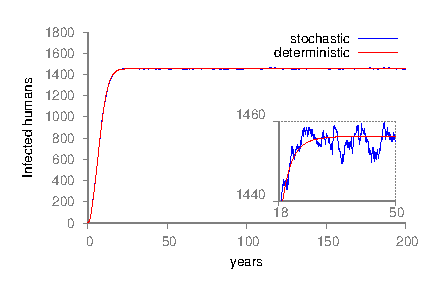
\includegraphics{%
			Sections/Section4/graphs/persistence/persistence_infected_humans.eps%
		}
	}
	\subfloat[][%
		Sotchastic bheavior of a infected animal 
		path.
		]%
	{%
		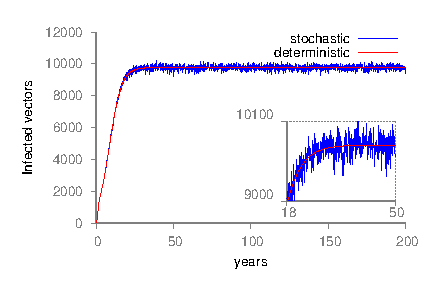
\includegraphics{%
			Sections/Section4/graphs/persistence/persistence_infected_vectors.eps%
		}
	}
	\caption{
		A sample path of the stochastic solution process
		of SDE \eqref{eq.8} under conditions of \Cref{theo:persist}.
	Parameters values in 
	\Cref{tbl:persistence_parameters}.
	}\label{fig:persistence_path}
\end{figure}

\begin{figure}[p]
	\centering
	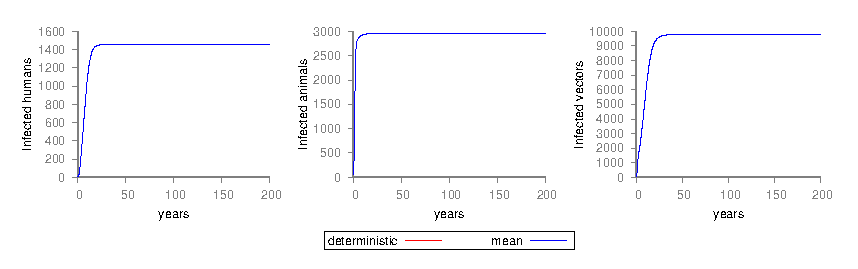
\includegraphics{%
		Sections/Section4/graphs/persistence/persistence_mean_population.eps%
	}
	\caption{
		Likening between deterministic solution and the mean of \num{10 000} 
		realizations of the stochastic solution process. As we see, our mean value 
		follows the deterministic profile.
	}
	\label{fig:mean_persistence}
\end{figure}
%%%%%%%%%%%%%%%%%%%%%%%%%%%%%%%%%%%%%%%%%%%%%%%%%%%%%%%%%%%%%%%%%%%%%%%%%%%%%%%%
%
%   Persistence Histograms at t = 200
%%%%%%%%%%%%%%%%%%%%%%%%%%%%%%%%%%%%%%%%%%%%%%%%%%%%%%%%%%%%%%%%%%%%%%%%%%%%%%%%
\begin{figure}[p]
	\centering
	\includegraphics{%
		Sections/Section4/graphs/persistence/persistence_histograms%
	}
	\caption{
		Histograms of \num{10 000} sample solution paths of SDE 
		\eqref{eq.8} under hypothesis of \Cref{theo:persist}
		and at fixed time $t=\num{200} ~\si{years}$.
	}
	\label{fig:persistence_histograms}
\end{figure}
%%%%%%%%%%%%%%%%%%%%%%%%%%%%%%%%%%%%%%%%%%%%%%%%%%%%%%%%%%%%%%%%%%%%%%%%%%%%%%%%
% Variance reduction.
%
%%%%%%%%%%%%%%%%%%%%%%%%%%%%%%%%%%%%%%%%%%%%%%%%%%%%%%%%%%%%%%%%%%%%%%%%%%%%%%%%
\begin{figure}[p]
	\centering
	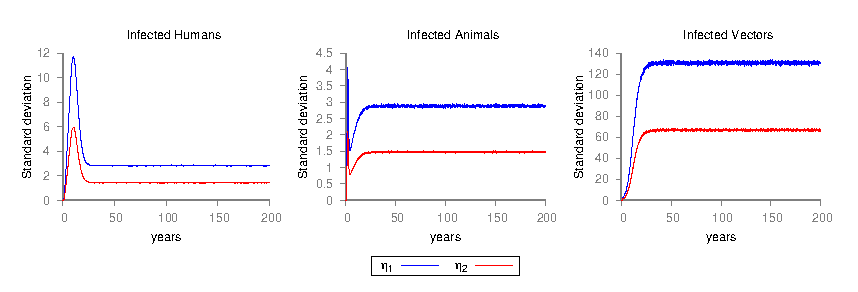
\includegraphics{%
		Sections/Section4/graphs/persistence/persistence_variance_population.eps%
	}
	\caption{
		The noise effect amplitude over variance. 
		of \num{10000} sample paths. Here we decrease the initial noise 
		intensities 
		$
			\eta_{1}:= 
			(
				\sigma_{z_h}^1,
				\sigma_{z_a}^1
			)
			=
			(
				\num{0.00395}, %~\si{bite.vector^{-1}.human^{-1}.year^{-1}}, 
				\num{0.00195} %~\si{bite.vector^{-1}.animal^{-1}.year^{-1}}
			)
		$ 
		until
		$
		\eta_{2}:= 
		(
			\sigma_{z_h}^2,
			\sigma_{z_a}^2
		)
		=
		(
			\num{0.002}, 
			%~\si{bite.vector^{-1}.human^{-1}.year^{-1}},
			\num{0.001}  
			%~\si{bite.vector^{-1}.animal^{-1}.year^{-1}}
		)
		$. As we see, this figure suggest that 
		noise intensity can modulates the solution 
		variance of SDE \eqref{eq.8}.
	}\label{fig:noise_variance_reduction}
\end{figure}